\documentclass[12pt]{beamer}
\usetheme{CambridgeUS}
\usepackage[utf8]{inputenc}
\usepackage[spanish]{babel}
\usepackage{amsmath}
\usepackage{amsfonts}
\usepackage{amssymb}
\usepackage{graphicx}
\author{Kevin Garcia - Alejandro Vargas}
\title{Modelo de regresión lineal múltiple}
%\setbeamercovered{transparent} 
%\setbeamertemplate{navigation symbols}{} 
%\logo{} 
%\institute{} 
%\date{} 
%\subject{} 
\begin{document}

\begin{frame}
\titlepage
\end{frame}

%\begin{frame}
%\tableofcontents
%\end{frame}

\begin{frame}
\frametitle{Análisis exploratorio de datos}
~\\ Para trabajar con la base de datos denominada 'cadata', generamos un número aleatorio con la ayuda del software R, el cuál nos arrojó el número 15529, por tanto nuestra base de datos final, quedo con las 9 variables (columnas) y con las filas desde la 15529 hasta la 16028.

~\\ El objetivo del estudio es ajustar un modelo de regresión para la variable 'Valor medio de la casa', tomando como variables explicativas las variables 'Ingreso medio','Edad media de la vivienda', 'Total de habitaciones','Total de dormitorios','Población','Hogares','Latitud' y 'Longitud'. 
\end{frame}

\begin{frame}
\frametitle{Análisis exploratorio de datos}
~\\ Previo al ajuste e interpretación del modelo, se llevo a cabo el respectivo análisis exploratorio de datos, para tener una idea de las descriptivas mas importantes de cada variable, su forma de distribución y su rango de valores.

\end{frame}

\begin{frame}
\frametitle{Variable 'Valor medio de la casa'}
\begin{figure}[!h]
    \begin{center}
        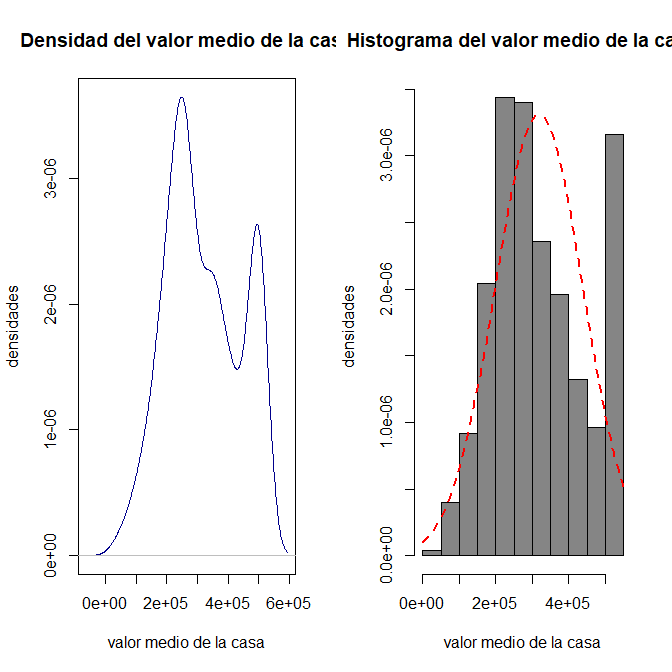
\includegraphics[width=10cm]{imagenes/1.png}
        \caption{Histograma y densidad de la variable 'Valor medio de la casa'}
        \label{fig:Densidad}
    \end{center}
\end{figure}
\end{frame}

\begin{frame}
\frametitle{Variable 'Ingreso medio'}
\begin{figure}[!h]
    \begin{center}
        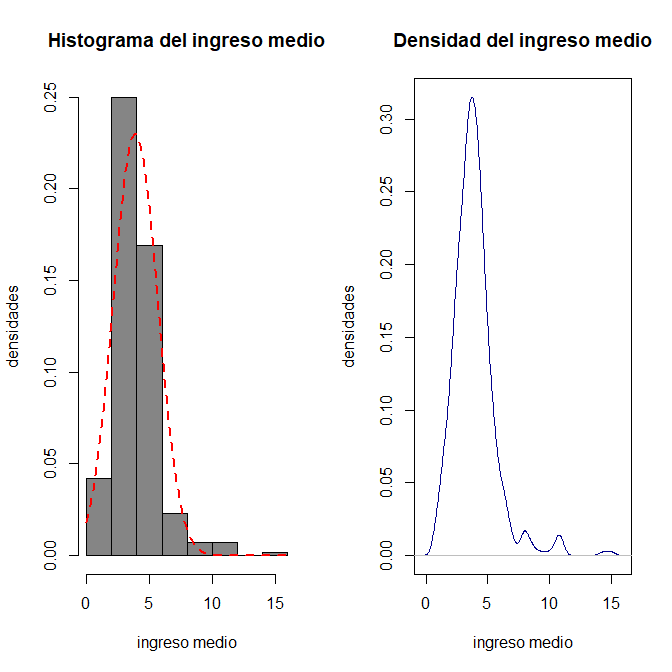
\includegraphics[width=10cm]{imagenes/2.png}
        \caption{Histograma y densidad de la variable 'Ingreso medio'}
        \label{fig:Densidad}
    \end{center}
\end{figure}
\end{frame}

\begin{frame}
\frametitle{Variable 'Edad media de la vivienda'}
\begin{figure}[!h]
    \begin{center}
        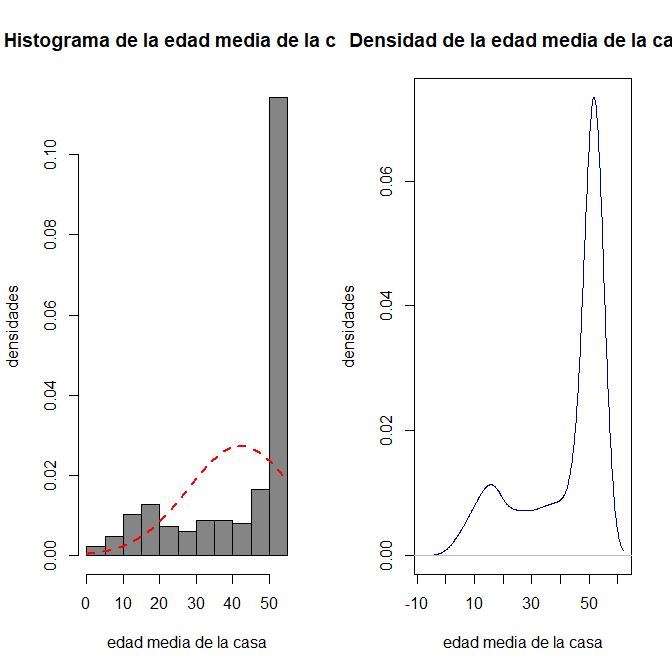
\includegraphics[width=10cm]{imagenes/3.png}
        \caption{Histograma y densidad de la variable 'Edad media de la vivienda'}
        \label{fig:Densidad}
    \end{center}
\end{figure}
\end{frame}

\begin{frame}
\frametitle{Variable 'Total de habitaciones'}
\begin{figure}[!h]
    \begin{center}
        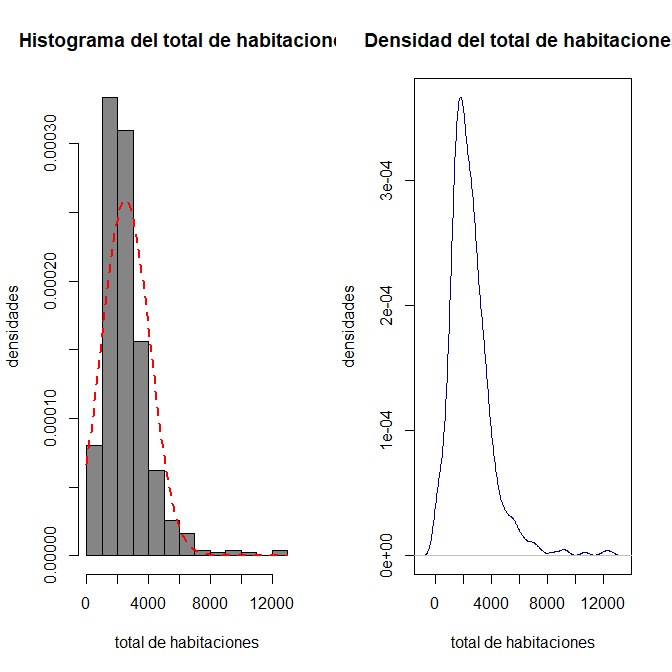
\includegraphics[width=10cm]{imagenes/4.png}
        \caption{Histograma y densidad de la variable 'Total de habitaciones'}
        \label{fig:Densidad}
    \end{center}
\end{figure}
\end{frame}

\begin{frame}
\frametitle{Variable 'Total de dormitorios'}
\begin{figure}[!h]
    \begin{center}
        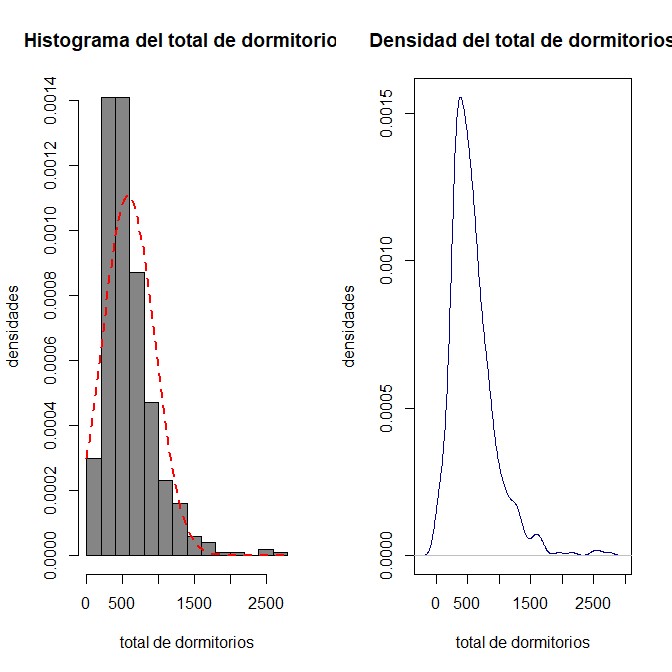
\includegraphics[width=10cm]{imagenes/5.png}
        \caption{Histograma y densidad de la variable 'Total de dormitorios'}
        \label{fig:Densidad}
    \end{center}
\end{figure}
\end{frame}

\begin{frame}
\frametitle{Variable 'Población'}
\begin{figure}[!h]
    \begin{center}
        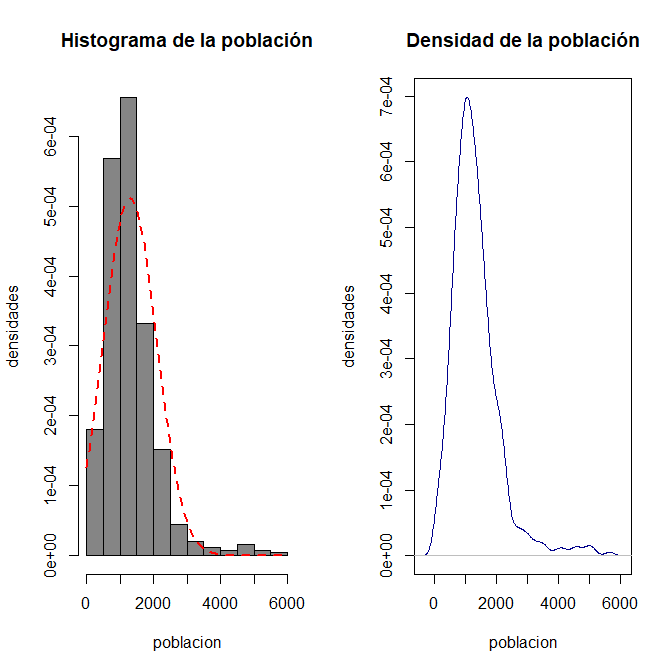
\includegraphics[width=10cm]{imagenes/6.png}
        \caption{Histograma y densidad de la variable 'Población'}
        \label{fig:Densidad}
    \end{center}
\end{figure}
\end{frame}

\begin{frame}
\frametitle{Variable 'Hogares'}
\begin{figure}[!h]
    \begin{center}
        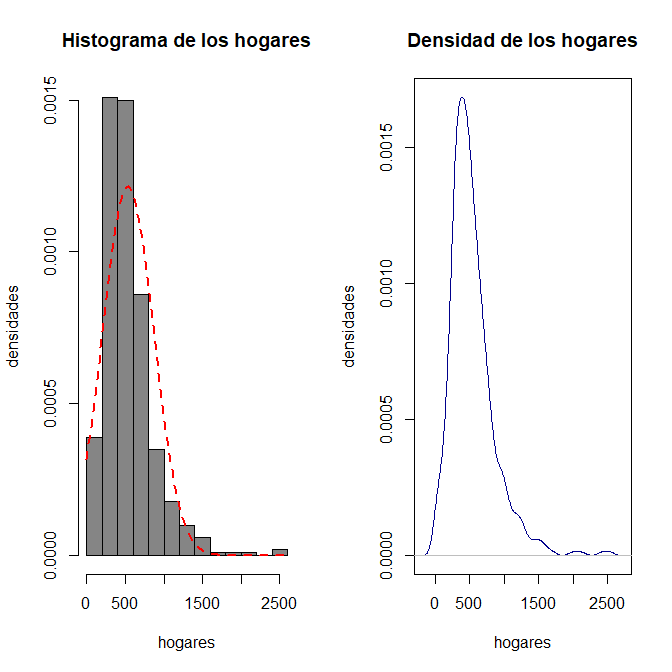
\includegraphics[width=10cm]{imagenes/7.png}
        \caption{Histograma y densidad de la variable 'Hogares'}
        \label{fig:Densidad}
    \end{center}
\end{figure}
\end{frame}

\begin{frame}
\frametitle{Variables 'Latitud'}
\begin{figure}[!h]
    \begin{center}
        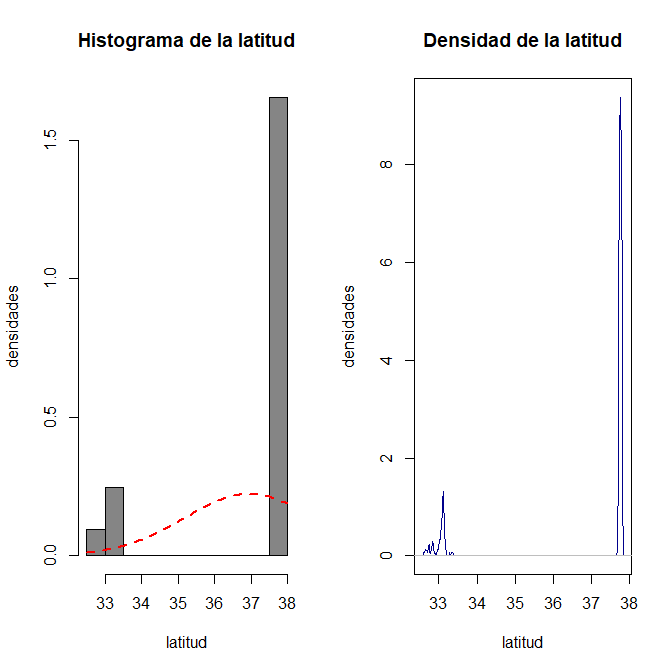
\includegraphics[width=10cm]{imagenes/8.png}
        \caption{Histograma y densidad de la variable 'Latitud'}
        \label{fig:Densidad}
    \end{center}
\end{figure}
\end{frame}

\begin{frame}
\frametitle{Variable 'Longitud'}
\begin{figure}[!h]
    \begin{center}
        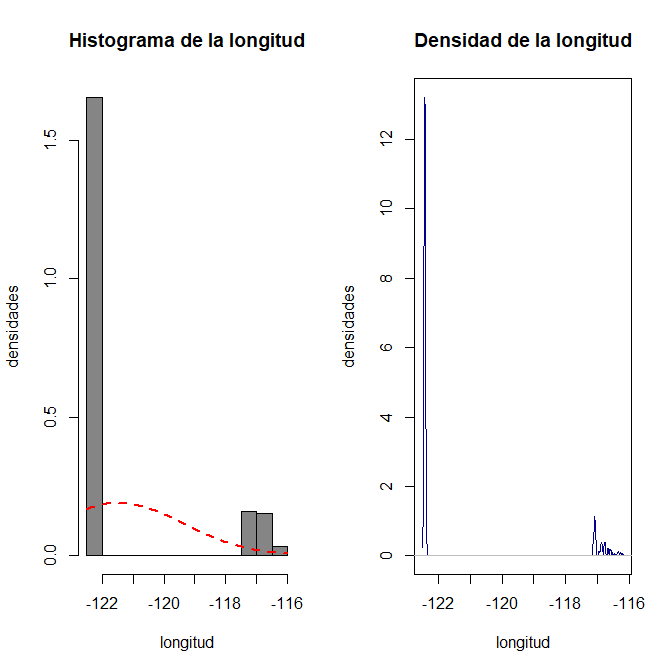
\includegraphics[width=10cm]{imagenes/9.png}
        \caption{Histograma y densidad de la variable 'Longitud'}
        \label{fig:Densidad}
    \end{center}
\end{figure}
\end{frame}
\begin{frame}
\frametitle{Modelo ajustado e interpretación}
\end{frame}
\end{document}